\documentclass[main.tex]{subfiles}
\begin{document}

\section{Sheet 2}

\subsection{Constant acceleration}

\subsubsection{Coordinate velocity}

We are given the position as a function of time, 
\begin{equation}
  x(t) = \frac{\sqrt{1 + \kappa^2 t^2} -1 }{\kappa }\,,
\end{equation}
%
and we can directly compute its derivative
%
\begin{equation}
  v(t) = \dv{x}{t} =
  \frac{\kappa t}{\sqrt{\kappa^2 t^2  + 1} }\,.
\end{equation}

It is clear from the expression that \(\abs{v} < 1\) for all times, while \(v\) approaches 1 at positive temporal infinity and \(-1\) at negative temporal infinity.

\begin{figure}[h]
    \centering
    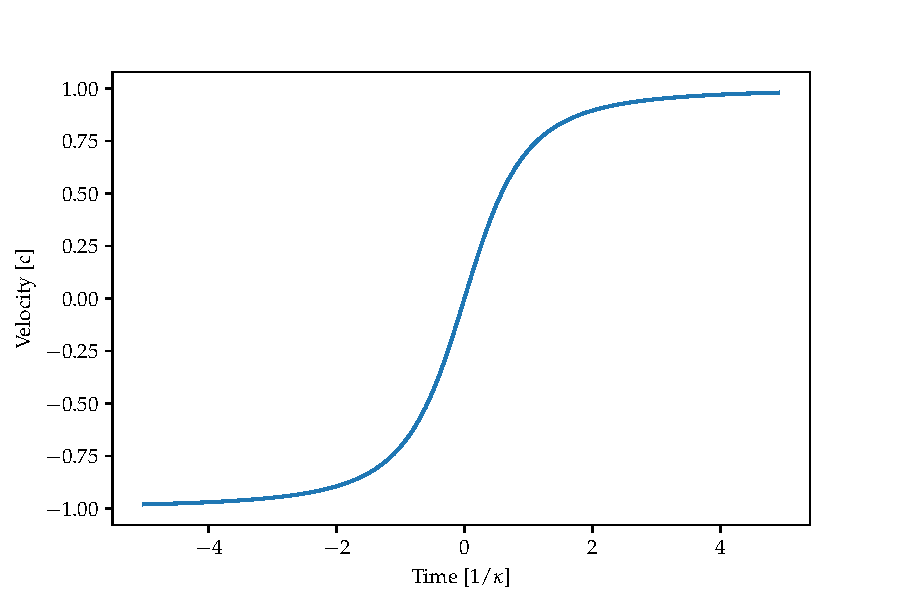
\includegraphics[width=\textwidth]{figures/velocity.pdf}
    \caption{Velocity as a function of coordinate time \(t\)}
    \label{fig:velocity-constant-acceleration}
\end{figure}

\subsubsection{Components of \(u^{\mu }\)}

The Lorentz factor \(\gamma \) is given by
%
\begin{equation}
  \gamma = \frac{1}{\sqrt{1-v^2}}
  = \frac{1}{\sqrt{1 - \frac{\kappa^{2} t^{2}}{\kappa^{2} t^{2} + 1} }}
  = \sqrt{\kappa^2 t^2 + 1} \,,
\end{equation}
%
therefore the four-velocity is given by:
%
\begin{equation}
  u^{\mu } =
  \begin{bmatrix}
  \gamma  \\
  \gamma v \\
  0 \\
  0
  \end{bmatrix}
  =
  \begin{bmatrix}
    \sqrt{\kappa^2 t^2 + 1}  \\
    \kappa t \\
    0 \\
    0
  \end{bmatrix}\,.
\end{equation}

\subsubsection{Proper time}

The relation between coordinate and proper time is given by the definition of the first component of the four-velocity: \(u^{0} = \dv*{t}{\tau} = \gamma \), therefore \(\dd{\tau } = \dd{t} / \gamma \).
Integrating this relation we get:
%
\begin{equation}
    \tau = \int \dd{\tau } 
    = \int \frac{\dd[]{t} }{\gamma }
    = \displaystyle \frac{\operatorname{arcsinh}{\left(\kappa t \right)}}{\kappa}\,,
\end{equation}
%
where the constant of integration is selected by imposing \(t = 0 \iff \tau = 0\).
Notice that, as we would expect, when expanding up to second order near \(t = \tau = 0 \) we have \(t \sim \tau \), since in that region the velocity is much less than unity.

The inverse relation is given by \(t = \sinh (\kappa \tau ) / \kappa \). Using this, we can write:
%
\begin{equation}
  x (t(\tau ))  =\frac{\cosh{\left(\kappa \tau \right)} - 1}{\kappa}\,.
\end{equation}

\subsubsection{Four-acceleration}

Now, we wish to compute the four-acceleration. There are many ways to approach this: an easy one is to simply find the explicit expression \(u^{\mu } (\tau )\) and to differentiate it. The expression we get is:
%
\begin{equation}
    a^{\mu } = \dv{}{\tau } u^{\mu } = \dv{}{\tau }   
  \begin{bmatrix}
    \sqrt{\sinh^{2}{\left(\kappa \tau \right)} + 1}
        \\
    \frac{\sqrt{\kappa^{2} t^{2} + 1} \sinh{\left(\kappa \tau \right)}}{\sqrt{\sinh^{2}{\left(\kappa \tau \right)} + 1}} \\
    0 \\
    0
  \end{bmatrix}
  =
  \begin{bmatrix}
    \frac{\sqrt{2} \kappa \sinh{\left(2 \kappa \tau \right)}}{2 \sqrt{\cosh{\left(2 \kappa \tau \right)} + 1}}
    \\
    \kappa \cosh \left(\kappa \tau \right)\\
    0 \\
    0
  \end{bmatrix}
\,,
\end{equation}
%
which is a bit unwieldy but it can be used to check two important facts: \(a^{\mu } a_{\mu } = \const \) and \(a^{\mu }u_{\mu } = 0\). The first of the two is:
%
\begin{equation}
    a^{\mu }a_{\mu } = -(a_0 )^2 + (a_1 )^2 =
    \kappa^{2} \cosh^{2}{\left(\kappa \tau \right)} - \frac{\kappa^{2} \sinh^{2}{\left(2 \kappa \tau \right)}}{2 \left(\cosh{\left(2 \kappa \tau \right)} + 1\right)}
    = \kappa^2 
\,,
\end{equation}
%
which tells us that the constant acceleration \(\sqrt{a^{\mu }a_{\mu }} = \kappa \).

Also, we verify the orthogonality to the four-velocity: 
%
\begin{equation}
  a^{\mu }u_{\mu } = 
  - \frac{\sqrt{2} \kappa \sqrt{\sinh^{2}{\left(\kappa \tau \right)} + 1} \sinh{\left(2 \kappa \tau \right)}}{2 \sqrt{\cosh{\left(2 \kappa \tau \right)} + 1}} + \kappa \sinh{\left(\kappa \tau \right)} \cosh{\left(\kappa \tau \right)}
  = 0
\,.
\end{equation}

\subsubsection{Local velocity \& acceleration}

We can apply a Lorentz boost corresponding to this velocity:
it will be given by the matrix:
%
\begin{equation}
  \left[\begin{array}{cccc}
  \gamma  & -v \gamma  & 0 & 0 \\ 
  -v \gamma  & \gamma  & 0 & 0 \\ 
  0 & 0 & 1 & 0 \\ 
  0 & 0 & 0 & 1
  \end{array}\right]
\,,
\end{equation}
%
where \(v\) and \(\gamma \) are those found before.
Without doing any calculations we could already say that the transformed velocity will be equal to the time-like unit vector, while the acceleration will be equal to \(\kappa \) times the unit \(x\)-directed vector.

The velocity becomes:
%
\begin{equation}
  \qty(u^{\mu})' =
  \left[\begin{array}{cccc}
    \sqrt{\kappa^2 t^2 + 1}  & -\kappa t  & 0 & 0 \\ 
    -\kappa t  & \sqrt{\kappa^2 t^2 + 1}  & 0 & 0 \\ 
    0 & 0 & 1 & 0 \\ 
    0 & 0 & 0 & 1
    \end{array}\right]
    \begin{bmatrix}
      \sqrt{\kappa^2 t^2 + 1}  \\
      \kappa t \\
      0 \\
      0
    \end{bmatrix} 
  = 
  \begin{bmatrix}
  1 \\
  0 \\
  0 \\
  0
  \end{bmatrix}
\,,
\end{equation}
%
as we expected.

The acceleration instead becomes:
%
\begin{equation}
  \qty(a^{\mu})' =
  \left[\begin{array}{cccc}
    \sqrt{\kappa^2 t^2 + 1}  & -\kappa t  & 0 & 0 \\ 
    -\kappa t  & \sqrt{\kappa^2 t^2 + 1}  & 0 & 0 \\ 
    0 & 0 & 1 & 0 \\ 
    0 & 0 & 0 & 1
    \end{array}\right]
    \begin{bmatrix}
      \frac{\sqrt{2} \kappa \sinh{\left(2 \kappa \tau \right)}}{2 \sqrt{\cosh{\left(2 \kappa \tau \right)} + 1}}
      \\
      \kappa \cosh \left(\kappa \tau \right)\\
      0 \\
      0
    \end{bmatrix}
  = 
  \begin{bmatrix}
  0 \\
  \kappa  \\
  0 \\
  0
  \end{bmatrix}
\,,
\end{equation}
%

\subsection{Fixed target collision}

\subsubsection{Center of mass momenta}

In the CoM frame, the momenta of the two protons are respectively \((E_p, \pm p, 0,0)^\top = m_p (\gamma, \pm v, 0, 0)\), where \(E_p^2 = m_p^2 + p^2\).
The total CoM energy is \(-(p^\mu _A + p^\mu _B )^2 = 2 m_p^2\).

\subsubsection{Center of mass velocity}

The momentum of particle \(B\) will be given by \(p^{\mu } = m_p u^{\mu } = (m_p \gamma , m_p \gamma v, 0, 0)^\top\). Therefore, \(\gamma v = p / m_p\). Solving this we get: 
%
\begin{equation}
  v = \frac{p}{m_p} \sqrt{\frac{1}{(p/m_p)^{2} + 1}} = \frac{p}{E_p}
\,,
\end{equation}
%

\subsubsection{Lab frame momenta}

The momentum of particle \(B\) in its own rest frame will just be \((m_p, 0, 0, 0)^\top\).
The momentum of particle \(A\) instead will be given by a boost in the \(x\) direction with velocity \(-v\):
%
\begin{equation}
  (p_A^\mu) _{\text{lab}} = 
  \left[\begin{array}{cccc}
  \gamma  & v \gamma  & 0 & 0 \\ 
  v \gamma  & \gamma  & 0 & 0 \\ 
  0 & 0 & 1 & 0 \\ 
  0 & 0 & 0 & 1
  \end{array}\right]
  \left[\begin{array}{c}
  E_p  \\ 
  p \\ 
  0 \\ 
  0
  \end{array}\right]  
  = \left[\begin{array}{c}
    \gamma E_p + v \gamma p  \\ 
    v \gamma E_p + \gamma p \\ 
    0 \\ 
    0
    \end{array}\right]  
  = \left[\begin{array}{c}
    m_p \frac{1+v^2}{\sqrt{1-v^2}}  \\ 
    2 \gamma p\\ 
    0 \\ 
    0
    \end{array}\right]
\,,
\end{equation}
%

\subsection{Weak field gravitational time dilation}



\end{document}